\documentclass{article}
\usepackage{tikz, pgfplots}
\usetikzlibrary{automata}
\usetikzlibrary{graphs,shapes.geometric} 
\usetikzlibrary{patterns}
\usepackage{graphicx, float, xcolor}
\usepackage{mathtools, mathrsfs, caption}
\usepackage{amsmath, amsfonts, amssymb, amsthm}
\captionsetup{font=small}
\numberwithin{equation}{section}

\usepackage{algorithm}
\usepackage[noend]{algpseudocode}
\newcommand\mycommfont[1]{\footnotesize\ttfamily\textcolor{blue}{#1}}
% \SetCommentSty{mycommfont}

% \SetKwInput{KwInput}{Input}                % Set the Input
% \SetKwInput{KwOutput}{Output}              % set the Output
\newcommand{\bigOh}[1]{\mathcal{O}\left(#1\right)}
\newcommand{\smallOh}[1]{\mathcal{o}(#1)}
\newcommand{\bigOmega}[1]{\Omega\left(#1\right)}
\newcommand{\smallomega}[1]{\omega(#1)}
\newcommand{\bigTheta}[1]{\Theta(#1)}
\newcommand{\curlyBrace}[1]{\left\{#1\right\}}
\newcommand{\roundBrace}[1]{\left(#1\right)}
\newcommand{\probsymb}[1]{\mathbb{P}\curlyBrace{#1}}
\usepackage{hyperref, biblatex}
\hypersetup{linkcolor=blue}
\usepackage[breakable,skins]{tcolorbox}
\tcbuselibrary{breakable}
\newcommand{\stepNumber}[1]{\textcolor{blue}{Step-(#1)}}
\usepackage{fancyhdr}
\pagestyle{fancy}
\chead{IEOR 6614: Homework 2}
\rhead{\textbf{UNI:} ag4808}
\lhead{02/27/2024}


\begin{document}

\section{Problem 1} %% problem 1
We are required to propose an infinite family of graphs for which the number of global min-cuts is equal to $n(n-1)/2$, where $n = |V(G)|$ is the number of vertices in the graph. This indicates that we should look for graphs such that,``if we pick any two vertices at random as $s$ and $t$ the $s-t$ min-cut is unique and also a `\textit{global min-cut}' for the graph."\\\\
Let us define the family of undirected graphs as $\{\varphi_k\}$ as follows: 
\begin{enumerate}
    \item $\varphi_1$ and $\varphi_2$ are not defined, as you need at least 3 vertices to make a cyclic graph. 
    \item $\varphi_3$ is a graph with 3 vertices connected by edges $\{(v_1, v_2), (v_2, v_3), (v_3, v_1)\}$ of unit capacity . 
    \item $\varphi_n$ is a cycle graph with $n$ vertices with each edge having unit capacity with vertices labelled as $v_i, \, \, \, \forall i \in [n]$ 
\end{enumerate}
\begin{figure}[H]
    \centering
    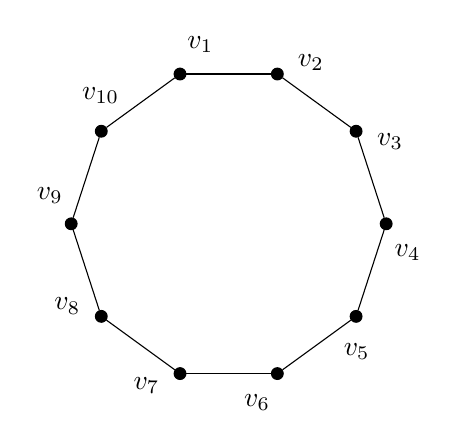
\begin{tikzpicture}
          \def\n{10} % Change this value to set the number of vertices
          
          % Define vertices
          \foreach \i in {1,...,\the\numexpr\n} {
            \coordinate (V\i) at ({\i*360/\n}:2);
            \node[circle, draw, fill=black, inner sep=1.5pt] (vertex\i) at (V\i) {};
          }
          
          % Draw edges
          \foreach \i in {1,...,\the\numexpr\n-1} {
            \pgfmathtruncatemacro{\next}{\i + 1}
            \draw (vertex\i) -- (vertex\next);
          }
          % Draw last edge to close the cycle
          \draw (vertex\n) -- (vertex1);
        
          % Label vertices
          \foreach \i in {1,...,\the\numexpr\n} {
            \pgfmathtruncatemacro{\angle}{-\i * 360 / \n + 135}
            \node at ({\angle}:2.3) {\(v_{\i}\)};
          }
    \end{tikzpicture}


    \caption{For example the graph corresponding to $\varphi_{10}$}
    \label{fig:enter-label}
\end{figure}
For the cycle graph $\varphi_n$, the max-flow value is 2 units for any pair of vertices $s$ and $t$ and hence by the max-flow min-cut theorem any min-cut will also have  a capacity of 2 units.\\\\
\textbf{Claim 1:} For the graph family $\varphi_{n}$ the number of undirected global min-cuts is $ = n(n-1)/2$ for $n\ge 3$. 
\begin{proof}
    As the cycle graph $\varphi_n$ has $n$ edges, and we get a cut of capacity 2 by disconnecting any two edges hence number of global-min-cuts equals the number of ways to select two edges from a set of $n$ edges, which is $n(n-1)/2$. 
\end{proof}
To show that for any graph $G = (V, E)$, the number of global minimum-cuts possible is at most $\binom{n}{2}$, we use ideas from Karger's randomized algorithm discussed in the lectures. The idea is to find a union-bound for the event of picking some global-min cut and then use trivial rules of probability to get an upper bound.\\\\
\textbf{Claim 2:} For any undirected graph $G = (V, E)$, with the size of the vertex set equal to $n$ we have at most $\binom{n}{2}$ global-min cuts. 
\begin{proof}
   We use the theorem proved in a modified manner, let $(X_k, V\setminus X_k)$ be a global min-cut then the event $\mathcal{E}_k$ on which Karger's algorithm returns this cut has probability at least $1/\binom{n}{2}$. We can then establish a union bound to get the bound on getting any global min-cut as follows, 
   \begin{equation}
       \label{e1}
       \mathbb{P}\biggl\{\bigcup_{k} \mathcal{E}_k\biggr\} = \sum_{k} \mathbb{P}\{\mathcal{E}_k\} \ge \frac{\{\text{number of global min-cuts}\}}{\binom{n}{2}}
   \end{equation}
   If we use the weak bound $\mathbb{P}\{\bigcup_{k} \mathcal{E}_k\} \le 1$, we get the desired result by cross-multiplying. (note, here we have used independence of the events, which is quite trivial by design of the algorithm) 
\end{proof}
\newpage
\section{Problem 2} %% problem 2
For part (a) - note that for graphs not satisfying the base case, we run Karger's algorithm partially (but independently) two times and recurse on the obtained contractions. So if we denote the run time of the algorithm on a graph with $n$ nodes as $T(n)$, then the following recursion holds:
\begin{equation}
    \label{e2}
    T(n) \le 2T\roundBrace{\frac{n}{\sqrt{2}}} + \bigOh{n^2}
\end{equation}
We can use \href{https://stanford-cs161.github.io/winter2022/assets/files/lecture3-notes.pdf}{Master theorem} (with $a=2$ $b=\sqrt{2}$ and $d = 2$) to get the solution of this recurrence as $T(n) = \bigOh{n^2\log(n)}$\\\\
For part (b) - We know that the probability of any global-min cut being preserved in contraction procedure is $\bigOmega{1/n^2}$ and in each step the algorithm reduced the problem size by $1/\sqrt{2}$ . If we denote the probability of success in a graph with $n$ - vertices as $p(n)$ then the following recursion holds
\begin{equation}
    p(n) = 1 - \roundBrace{1 - \frac{1}{2}p\roundBrace{\frac{n}{\sqrt{2}}}}^2
\end{equation}

\noindent The intuition being that $\frac{1}{2}p(n/\sqrt{2})$, is the probability that one of the two independent runs succeed, which means that $\roundBrace{1 - \frac{1}{2}p(n/\sqrt{2})}^2$ is the probability that both of the runs fail in preserving the right global min-cut. \\\\
\textbf{Claim 1:} $p(n) \ge \frac{1}{\log(n)}$
\begin{proof}
    We can use induction to prove this claim, let us first expand the terms in our recursive formulae as follows, 
    \begin{equation}
        \begin{split}
            p(n) &= 1 - \roundBrace{1 - \frac{1}{2}p\roundBrace{\frac{n}{\sqrt{2}}}}^2\\\\
            &= 1 - \roundBrace{1+\frac{1}{4}p\roundBrace{\frac{n}{\sqrt{2}}}^2 - p\roundBrace{\frac{n}{\sqrt{2}}}}\\\\
            &= p\roundBrace{\frac{n}{\sqrt{2}}} - \frac{1}{4}p \roundBrace{\frac{n}{\sqrt{2}}}^2
        \end{split}
    \end{equation}
Note that $f(x) = x - x^2/4$  is an increasing function for $x \le 1$. By our induction hypothesis we know that $p(n/\sqrt{2}) \ge  1/\log{(n/\sqrt{2})}$ using these two facts we have the following, 
\begin{equation}
\label{e3}
    p(n) \ge \frac{1}{\log(n/\sqrt{2})} - \frac{1}{4\log^2(n/\sqrt{2})}
\end{equation}
It is enough to show that the right hand side of inequation \ref{e3} is greater than $1/\log(n)$. We proceed as follows, 
\begin{equation}
\begin{array}{ccc}
     &\frac{1}{\log(n/\sqrt{2})} - \frac{1}{4\log^2(n/\sqrt{2})} &\ge \frac{1}{\log{n}}  \\\\
     \leftrightarrow& \frac{\log{n} - \frac{1}{2}}{\log{n}} + \frac{1}{4 \log{n/\sqrt{2}}} &\le 1\\\\
\leftrightarrow& \frac{1}{4 \log{n/\sqrt{2}}}& \le \frac{1}{2\log{n}}
\end{array}
\end{equation}
The last inequality is true for $n\ge 2$ (as the base case is $n\le 6$ we need not worry ). Hence the induction holds and we are done with the proof. 

    
\end{proof}
\noindent For part (c) - if we run the algorithm for  $K = \log^2 n$ independent runs then the probability of success will be at least, 
\begin{equation}
    \probsymb{\mathcal{E}} \ge 1 - \roundBrace{1 - \frac{1}{\log n}}^{\log^2 n} \ge \roundBrace{1- \frac{1}{n}}
\end{equation}
\textbf{Claim 2:} $\probsymb{\mathcal{E}} 
\ge \roundBrace{1- \frac{1}{n}}$
\begin{proof}
    We use the taylor series expansion of $f(x) = e^{-x}$ to conclude that $e^{-x}\ge (1-x)$ ; now put $x = \log(n)$ and raise both sides to the power of $\log^2(n)$, this gets us $1/n \ge \roundBrace{1 - \frac{1}{\log n}}^{\log^2 n}$, which is sufficient to conclude the proof. 
\end{proof}
\newpage
\section{Problem 3} %% problem 3
For part (a) - the choice of the vertex $v_1$ should be arbitrary according to the given relation in the problem. We have the following simple procedure.
\begin{algorithm}[H]
    \caption{ORDER($G, v_1$)}
    \begin{algorithmic}[1]
        \State $S\leftarrow\{v_1\}$ 
        \ForAll{$i \leftarrow 2$ to $n$}
            \State Choose $v_i$ such that $v_i = \arg\max_{v \in V\setminus S} \sum_{x \in S} u(\{x, v\})$ 
            \State $S\leftarrow S\cup \{v_i\}$ 
        \EndFor
    \end{algorithmic}
\end{algorithm}
It can be seen that we iterate for $\bigOh{n}$ iterations of the outer loop and in each iteration the work done is linear in the size of $V\setminus S$, so the work done over all iterations is $\bigOh{n^2}$. \\\\
For part (b) - we need to show that given the ordering $v_1, \dots, v_n$ the minimum cut separating $v_n$ and $v_{n-1}$ is $(V\setminus\{v_n\}, v_n)$ . (alternate form of what was given in the question)\\\\
\textbf{Claim 1:} For any triplet $\langle v_i, v_j, v_k\rangle$ of distinct vertices (i.e. - $v_i\not=v_j\not=v_k$) the following holds true, 
\begin{equation}
    \label{e4}
    \Lambda(v_i, v_k) \ge \min\{\Lambda(v_k, v_j), \Lambda(v_i, v_k)\}
\end{equation}
Where $\Lambda(x, y)$ denotes the value of the min $x-y$ cut in the graph. \\\\
\begin{proof}
Let $(A, V\setminus A)$ be the $v_i-v_j$ min-cut in the graph with $v_i \in A$. Now if $v_k \in A$ then $\Lambda(v_i, v_j) \ge \lambda(v_k, v_j)$ since $A$
is also a $v_k-v_j$ cut. If $v_k\notin A$ then $\Lambda(v_i, v_j) \ge \Lambda(v_i, v_k)$ since $A$ is also a $v_i-v_k$ cut. Hence we just take the minimum of these two to get the result.
\end{proof}
\noindent\textbf{Claim 2}: Given the ordering $v_1, \dots, v_n$ the minimum cut separating $v_n$ and $v_{n-1}$ is $(V\setminus\{v_n\}, \{v_n\})$ 
\begin{proof}
    As $\Lambda(v_{n-1}, v_n)$ is a min-cut value we have, 
    \begin{equation}
        \Lambda(v_{n-1}, v_n) \le \sum_{e \in \delta^+(\{v_n\})} u(e)
    \end{equation}
    We need to prove the reverse, so let us use induction on the number of edges and nodes in the graph. 
    \begin{enumerate}
        \item For the base case take $n=2$ and $m=1$, then the claim in trivially true. 
        \item For the inductive step, 
        \item[] \begin{enumerate}
                    \item Case 1: there is an edge $e$ from $v_{n-1}$ to $v_n$. Then we remove that edge from the graph and call the new graph $G'$. Let $u(\delta(S))$ be the edges in $G'$ that have exactly one end in $S$. Then the original ordering is still valid for $G'$ and, 
                    \begin{equation}
                        \begin{split}
                            u(\delta(\{v_n\})) &= u(\delta'(\{v_n\})) + u(e)\\
                            &= \Lambda'(v_{n-1}, v_n) + u(e)\\
                            &= \Lambda(v_{n-1}, v_n)
                        \end{split}
                    \end{equation}
                    \item[] The second inequality follows from induction and the last inequality is due to the fact that any $v_{n-1}-v_n$ cut in $G'$ has the value equal to $v_{n-1}-v_n$ cut in $G$ minus the capacity of $e$. 
                    \item Case 2: there is no edge $e$ from $v_{n-1}$ to $v_n$. In this case we first formulate two graphs $G'$ and $G''$ such that $G' \leftarrow G - v_{n-1}$ and $G''\leftarrow G - v_n$. Then for $G'$ the ordering $v_1, \dots, v_{n-2}, v_n$ is still valid and by the inductive hypothesis we have, 
                    \begin{equation}
                        \begin{split}
                            u(\delta(\{v_n\})) &= u(\delta'(\{v_n\}))\\
                        &= \Lambda'(v_{n-2}, v_n)\\
                        &\le \Lambda(v_{n-2}, v_n)
                        \end{split}
                    \end{equation}
                    \item[] The last inequality is true because all capacities are non-negative hence the cut separating $v_{n-2}$ and $v_n$ in $G$ has a value at least the cut separating $v_{n-2}$ and $v_n$  in $G'$. 
                    \item[] 
                    \item[] Similarly for the graph $G''$ note that $v_1, \dots, v_{n-1}$ is a valid ordering and via the inductive hypothesis, 
                    \begin{equation}
                        \begin{split}
                            u(\delta(\{v_n\})) &\le u(\delta(\{v_{n-1}\}))\\
                            &=u(\delta''(\{v_{n-1}\}))\\
                            &= \Lambda''(v_{n-2}, v_{n-1})\\
                            &\le \Lambda(v_{n-2}, v_{n-1})
                        \end{split}
                    \end{equation}
                \end{enumerate}
            \item[] Now by the claim above we have, 
            \begin{equation}
                \begin{split}
                     \Lambda(v_{n-1}, v_{n}) &\ge \min(\Lambda(v_{n-2}, v_{n-1}), \Lambda(v_{n-2}, v_n))\\
                     &\ge u(\delta(\{v_{n}\}))
                \end{split}
            \end{equation}
            \item[] Hence the inductive hypothesis holds and the cut $(V-\{v_{n}\}, \{v_n\})$ is the minimum $v_{n-1}-v_n$ cut if the vertices are ordered by the algorithm above and we are done.   
    \end{enumerate}
    \end{proof}
    \noindent For part (c) - Consider the following algorithm for the global min-cut problem on an undirected graph $G$, 
    \begin{algorithm}[H]
        \caption{MINCUT(G)}
        \begin{algorithmic}[1]
            \State Pick any vertex as $v_1$
            \State Run \texttt{ORDER}($G, v_1$) to order the vertices. 
            \Statex
            \If{we have only two vertices}
                \State \Return{$\delta(\{v_n\})$}
            \Else
                \State Shrink $v_n$ and $v_{n-1}$ to obtain $G'$
                \State \Return{$\min\{\delta(\{v_n\}), \texttt{MINCUT}(G')\}$}
            \EndIf
        \end{algorithmic}
    \end{algorithm}
\noindent \textbf{Claim 3:} The algorithm above computes the correct undirected minimum-cut of the given graph $G$. 
\begin{proof}
    The minimum-cut of the graph can either be a $v_{n-1}-v_n$ cut or it is not. In the first case when it is the minimum cut, the algorithm correctly returns the correct cut due to the property of the ordering algorithm (see the previous claim). If it is not then in the minimum-cut the two vertices remain in the same partition and hence shrinking doesn't alter the minimum-cut and we recursively call the algorithm. 
\end{proof}
\noindent \textbf{Claim 4:} The algorithm $\texttt{MINCUT(.)}$ works in time $\mathcal{O}(n^3)$, where $n=|V(G)|$. 
\begin{proof}
    In each recursive call we have to order the vertices which makes us spend $\bigOh{n^2}$ time and we only recurse at most once. Also since the algorithm removes one vertex by shrinking each call, we can reduce the size of the graph at most $(n-2)$ times, this means we do $\bigOh(n^3)$ total work. 
\end{proof}
\newpage 
\section{Problem 4} %% problem 4
Let $M$ be a $k\times k$ sub-matrix of $A$. Then we define a matrix $U \in \{0, 1, -1\}^{k\times k}$ as follows, 
\begin{equation}
    U_{ik} = \begin{cases}
        1, \, \, \,\, \, \, \, \,  if \, \, k=i\\
        -1,\, \, if \,\, k=(i+1)\\
        0, \, \, else
    \end{cases}
\end{equation}
Note that $|U|=1$ (since by applying elementary transformations it can be converted into the identity matrix). Now consider the matrix product $MU$, and notice that each row of this product matrix can have at most one $+1$ and at most one $-1$ entry (due to the consecutive-ones property). Using the theory seen in lectures we can say that $MU$ is totally-unimodular and hence the following holds, 
\begin{equation}
    |M| = |MU| \in \{0, 1, -1\}
\end{equation}
As the matrix $M$ was an arbitrary $k\times k$ sub-matrix we can conclude that the above analysis holds true for all sub-matrices and for all valid $k$. Hence the matrix is totally-unimodular.\\\\
% For the second part assume that we have ordered the vertices such that $v_1\le v_2 \le \dots \le v_n$ such that if $(v_i, v_j) \in E$, then $(v_i, v_k), \, (v_k, v_j)\in E$ for all $i < k < j$. If we denote the node-arc incidence matrix (unsigned) as $A$ then the maximum stable set problem is given by the following integer program, 
% \begin{equation}
%     \begin{array}{crl}
%        \max&  1^\top x&  \\
%        & A^\top x &\le 1\\
%        & x &\in \{0, 1\}^{|V|}
%     \end{array}
% \end{equation}
% If it was possible to show that using the ordering above we can write $A$ or $A^\top$ as a matrix with consecutive-ones property then by total-unimodularity we know that the vertices are all integral and we can use the linear-programming techniques to solve the problem efficiently. All that remains is to show that $A$ or $A^\top$ has the consecutive-ones property. 
%%%%%%%%%%%%%%%%%%%%%%%%%%%%%%%%%%(doubt)%%%%%%%%%%%%%%%%%%%%%%%%%%%%%%%%%%%%%%
For part (b) - assume that we are given a graph $G$ with the given property, we show two things: 
\begin{enumerate}
    \item The maximal-clique based formulation of the Maximum-Stable set problem has consecutive ones property. 
    \item The constraint matrix corresponding to maximal-clique formulation has linear-size. 
\end{enumerate}
A clique in an undirected graph is a sub-graph in which all vertices are adjacent to each other. A clique which cannot be extended by adding more vertices is called the maximal-clique. Based on this structure we know that amongst each maximal clique we can pick at-most one vertex. Let $x_v\in \{0, 1\}$ be the binary variable representing whether the vertex is included in the stable set or not then, 
\begin{equation}
    \begin{array}{crl}
        \max & \sum_{v \in V} x_v &\\
         & \sum_{v\in S} x_v &\le 1, \, \, \, \, S \text{ is a maximal-clique in G}\\
         & x_v&\in \{0, 1\}
    \end{array}
\end{equation}
\textbf{Claim 1:} For each index $i$, pick the index $j$ farthest from $i$ in the ordering such that $j > i$ and $(v_i, v_j) \in E$, then vertices $\{v_i, v_{i+1}, \dots, v_j\}$ form a maximal-clique. 
\begin{proof}
    First we prove that these vertices form a clique, we know by the property that every vertex $v_k\in \{v_{i+1}, \dots, v_{j-1}\}$ is adjacent to $v_i$ and $v_j$. Fix a $k$, and recurse on vertices $\{v_{i+1}, \dots, v_{k-1}\}$ and $\{v_{k+1}, \dots, v_{j-1}\}$, and you get all the vertices are adjacent to each other.\\\\
    Now if this clique was not maximal then there exists a bigger clique involving all these vertices, this implies we either have some some $v_j'>v_j$ such that adding it to the set increases the clique size, but this is a contradiction to the way we chose $j$ for a given $i$. 
 \end{proof}
 \noindent \textbf{Claim 2:} The constraint matrix of this IP has consecutive ones property. 
 \begin{proof}
     For each maximal-clique, we have one inequality and by previous claim each maximal-clique can be uniquely identified for a given $i$ as vertices $v_i\le v_{i+1}\le\dots\le v_{j} $ ; hence the row corresponding to this constraint has 1's on consecutive indices from $i\text{ to }j$ and zero elsewhere ; hence the IP constraint matrix has consecutive ones property (it is totally-unimodular and all the vertices of the polytope are integral). 
 \end{proof}
 \noindent \textbf{Claim 3:} A graph with the property given above can have finitely many maximal-cliques and hence the LP can be solved efficiently via ellipsoid method. 
 \begin{proof}
     For a fixed $i$, we can find the maximal clique containing it by selecting the farthest vertex from it. Hence if you start from $v_1$ finding maximal-cliques they will form disjoint intervals of such indices. And you can fit at most $n$ disjoint intervals ; this means at most $n$ inequalities. 
 \end{proof}
\newpage
\section{Problem 5} %% problem 5
Let $G$ be a connected graph (with no isolated vertices) and let $M$ be a maximum-cardinality matching. Let $\mu(G)$ be the size of $M$ and $\beta(G)$ be the size of the minimum edge cover. We want to show that for every $M$, we can find an edge cover $C$ such that $|C| = \beta(G)$\\\\
The matching has $\mu(G)$ edges hence it covers $2\mu(G)$ vertices, this means that $|V| - 2 \mu(G)$ vertices of the graph are unmatched. As the graph $G$ is connected, we can cover the unmatched vertices by adding a set of edges $E$ to $\mu(G)$ of size $|V| - 2 \mu(G)$ (as each unmatched vertex must be adjacent to some matched vertex else as the graph has no isolated vertices if all neighbours were unmatched $M$ could be extended to a bigger matching, adding such an edge suffices). Hence, the set $E\cup M$ has a size of $|V| - \mu(G)$ and is an edge-cover. If we prove that it is a minimum edge-cover we get an algorithm to construct the same provided any $M$. \\\\
\textbf{Claim 1:} The edge cover $M\cup E$ created above is a minimum edge-cover for the graph $G$. 
\begin{proof}
    Note that the minimum edge cover cannot contain a cycle (else elimination of an edge on a cycle will lead to a smaller edge cover). Hence, we can assert that it must be a union of tree-graphs, i.e. - forest. Using the proposition proved in the lectures (about edges in a forest with $k$-components) we have the number of components in the forest induced by the minimum edge-cover to be $|V| - \beta(G)$. If we pick a single edge from everyone of these components we get a matching $M'$ of size $|V| - \beta(G)$. As $M$ is a maximum-matching we have $\mu(G) \ge |V| - \beta(G)$, or $\beta(G) \ge |V| - \mu(G)$\\\\
    But then as $M\cup E$ has the size $|V| - \mu(G)$ equality holds and hence it must be a minimum edge-cover. 
\end{proof}
\begin{algorithm}[H]
    \caption{EXTEND($M, \, G$)}
    \begin{algorithmic}[1]
        \State $E \coloneqq \{\}$
        \ForAll{$v \in V$ such that $v$ is unmatched}
            \State To $E$, add edges with one end as $v$ and the other a matched vertex. 
        \EndFor
        % \State Run cycle-elimination on $E$ (to remove unecessary edges)
        \State \Return $E$
    \end{algorithmic}
\end{algorithm}
\newpage
\section{Problem 6} %% problem 6
Given $k$ goods each having a source ($s_i$) and a sink ($t_i$) node. The network edges have a positive upper bound on the total flow. Let us define the following, 
\begin{itemize}
    \item $val(f_i) = \sum_{e \in \delta^+(s_i)}, \, \, \, \forall i \in [k]$, as the value of flow of the $i^{th}$-commodity. 
    \item $u_a > 0$, is the capacity of an arc $a$ of the flow-network. 
    \item $ex_f(v)$ is the difference of the outflow and inflow of all commodities at a node $v$.
\end{itemize}
The integer program is as follows, 
\begin{equation}
    \label{E6}
    \begin{array}{rlc}
    \\
        \max_f& \sum_{i\in[k]}\sum_{e \in \delta^+(s_i)} f_i(e) &  \\\\
         s.t.& \sum_{e \in \delta^+(v)} f_i(e) - \sum_{e \in \delta^-(v)} f_i(e)=0 &\forall v \notin\{s_i, t_i\}, \, \, \forall i \in [k]\\\\
         &\sum_{i\in [k]} f_i(e)\le u_e & \, \, \, \, \forall e \in E\\\\
         &f\in \mathbb{Z}_{\ge 0}
    \end{array}
\end{equation}
If we relax the integrality constraints in \ref{E6} then we need to check if the resulting linear-program has an integral solution or not. The intuition say it is not and we should be able to show that the constraint matrix is not totally-unimodular for this case. It is sufficient to show an example for which all data is integer but constraint matrix is not totally unimodular. Consider the following six-node graph, 
\begin{figure}[H]
    \centering
    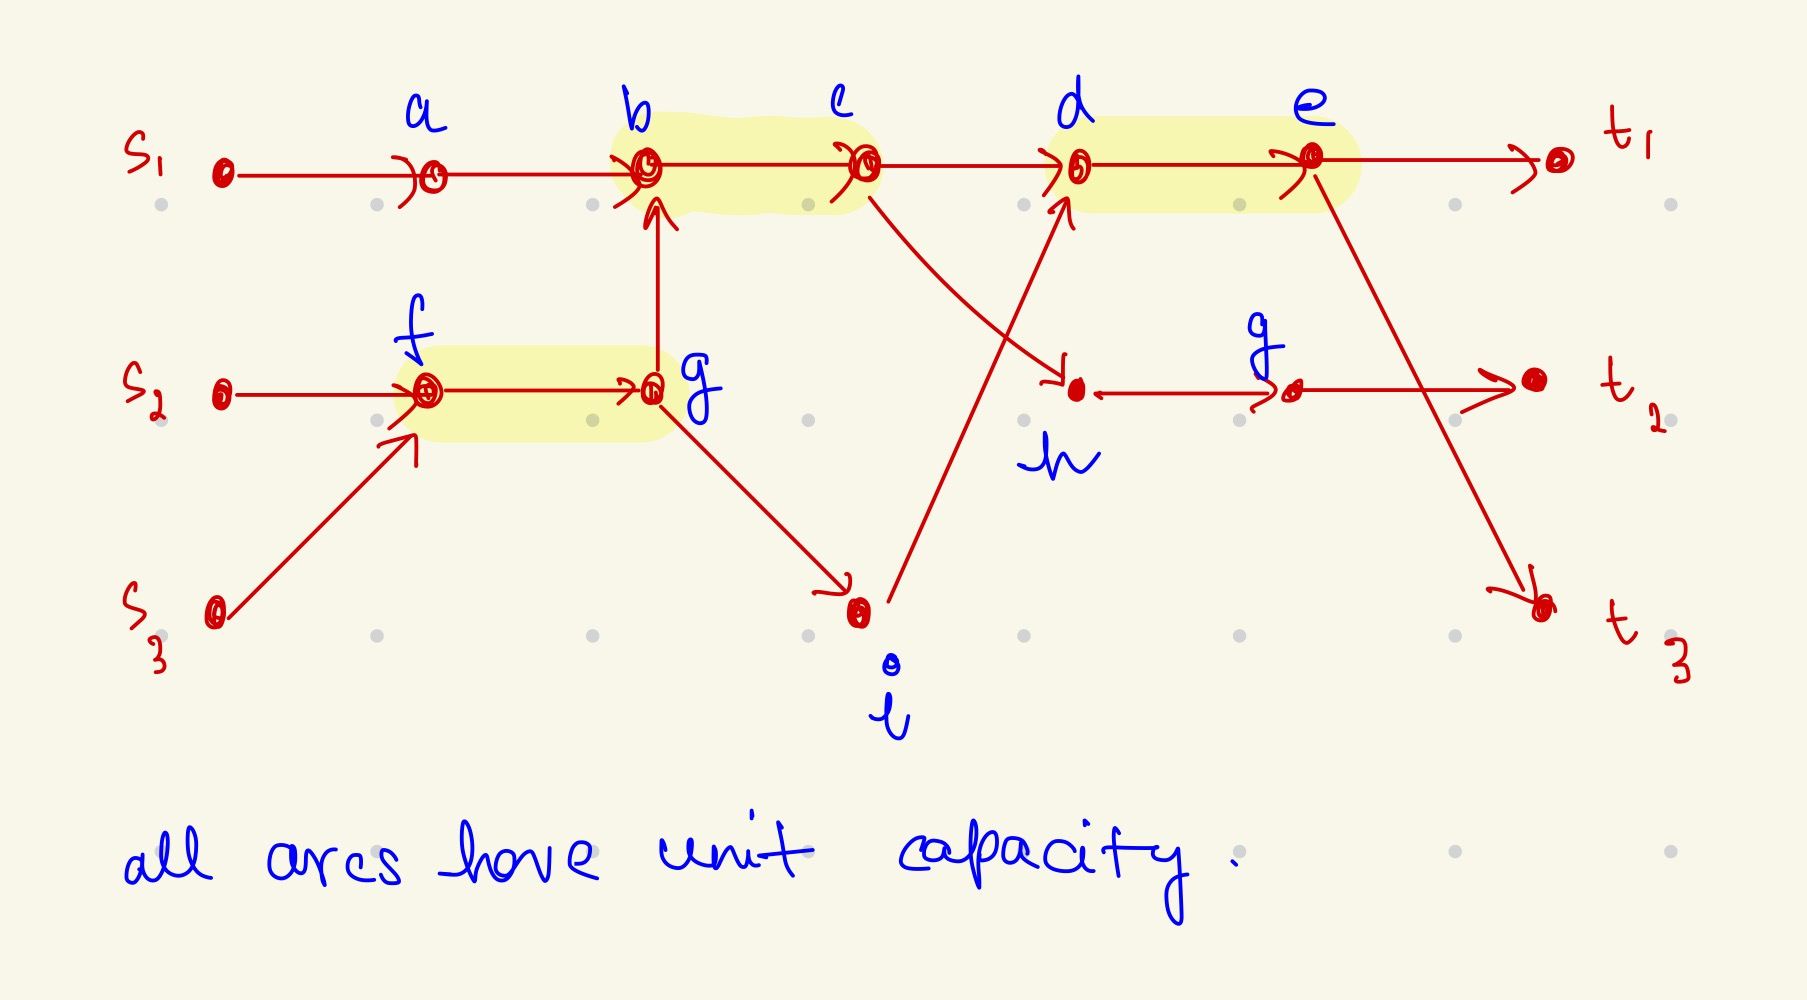
\includegraphics[width = 0.50\linewidth]{resources/HW2Q6.jpeg}
    \caption{Counter-example to integrality}
    \label{fig:enter-label}
\end{figure}
\noindent Note that in the above graph all data is integer still due to the coupling constraint on edge $(u, v)$, the constraint matrix is not totally unimodular and the optimal solution turns out to be fractional i.e. - $(f_1 = 0.5, f_2 = 0.5, f_3 = 0.5)$ ; any integral solution will have one unit of flow out of some vertex which will mandate the flow out of the other two vertices to be 0 due to coupling edges (yellow).
\newpage
\section{Problem 7} %% problem 7
%%%%%%%%%%%%%%%%%%%%%%%%%%%%%%%%%%%%%%%(DOUBT)%%%%%%%%%%%%%%%%%%%%%%%%%%%%%%%%%%%%%%%%%%%
For part (a) - As we have $n$ variables, the vertex of the polyhedron needs at least $n$-active linearly independent constraints. Hence let us denote the $n\times n$ integral basis matrix formed by these tight constraint as $B$. Note that the solution for $x$ can be written as, 
\begin{equation}
    x^* = B^{-1}b
\end{equation}
Due to the given property we know that $B$ has a determinant value equal to $0, -1, +1$. As the constraints are linearly independent the determinant cannot be null and hence the inverse exists and is integral as determinant, entries of the co-factor matrix are integral.\\\\
For part (b) - take the example polyhedron with $n=2$, as below
\begin{equation}
    P = \{(x_1, x_2) | x_1 + x_2 \le 6 \; 2x_1+x_2 \le 6\}
\end{equation}
\begin{figure}[H]
    \centering
    \begin{tikzpicture}[scale = 0.5]
    % Axis
    \draw[->] (-6,0) -- (8,0) node[right] {$x_1$};
    \draw[->] (0,-6) -- (0,8) node[above] {$x_2$};
    
    % Shading
    \fill[pattern=north west lines,pattern color=red!50] (-3,9) -- (0,6) -- (3, 0) -- (4, -2) -- cycle;
    
    % Vertices and inequalities
    \node[below left] at (0,0) {$(0,0)$};
    \node[above right] at (0,6) {$(0, 6)$};
    % \node[below] at (3,3) {$x_1 + x_2 \leq 6$};
    % \node[above right] at (6,0) {$x_1 \leq 6$};
    
    % Intersection points
    \fill (0,6) circle (1.2pt);
    
    % Draw lines
\end{tikzpicture}
    \caption{Graph for $P$ (shaded red), vertex at $(0, 6)$}
    \label{fig:enter-label}
\end{figure}
\noindent It satisfies the definition given above, but node the constraint matrix is not totally unimodular (as one of the $1\times 1$ sub-matrix has determinant 2)
\newpage
\section{Problem 8} %% problem 8
For part (a) - consider the dual of the max-flow LP, we know from the definition of a TU matrix that all its sub-matrices also need to be TU. The matrix $A$ is TU and hence the matrix $A'$ is TU. If we can prove that transposing preserves unimodularity then the augmented matrix, 
\begin{equation}
    U = \begin{bmatrix}
        A'^\top& I
    \end{bmatrix}
\end{equation}
is also TU and we are done (as in the class we had seen augmenting with identity matrix preserves total-unimodularity).\\\\
\textbf{Claim 1:} Transpose of a TU matrix is also TU. 
\begin{proof}
    If we pick any square sub-matrix of the transpose of a TU matrix, it will be the transpose of a square sub-matrix of the TU-matrix (as transposing just interchanges rows and column indices). We know that any square sub-matrix of the TU-matrix has determinant equal to$ 0, -1$, or  $+1$. This means that it's transpose also has the same determinant value. This implies that every square sub-matrix of the transpose has determinant equal to $0, -1,\text{or } +1$ and by definition of TU matrices we are done. 
\end{proof}
As the constraint matrix of the dual problem is TU, and $c$ is integral we can say that the polyhedron defined by them has integer vertices. \\\\
For part(b) - The inequality given in the problem holds for all vertices different from $s$, $t$. To extend it first assume that $v=s$ and $w\not=t$, then the constraint corresponding to edge $(s, w)$ in the dual is $\overline{y}(w) + \overline{\pi}(s, w) \ge 0$ ( as $A'$ doesn't have the row corresponding to $A$). Taking $\overline{y}(s)=0$, we get the extension needed. Similarly for every arc of the form $(w, t)$, such that $w\not=s$, we have $-\overline{y}(w) +\overline{\pi}(w, t) \ge 1$, if we define  $\overline{y}(t)=-1$, we are done. (other cases follow similarly)\\\\
For part (c) - Let $S = \{v \in V: \overline{y}(v) \ge 0\}$, then $S\subseteq V$ and $s \in S$ and $t\notin S$, hence $S$ is a valid cut. Let $F = \{(v, w) \in E : v\in S, \, w\notin S\}$ we have, 
\begin{equation}
    cap(S) = \sum_{(v, w)\in F} u(v, w) \le \sum_{(v, w)\in F} u(v, w) + \sum_{(v, w)\in E\setminus F} u(v, w)\overline{\pi}(v, w)
\end{equation}
Here the inequality holds due to non-negativity of $u$ and $\overline{\pi}$, \\\\
\textbf{Claim 2:} The following is true, 
\begin{equation*}
    \sum_{(v, w)\in F} u(v, w) \le \sum_{(v, w)\in F} u(v, w)\overline{\pi}(v, w)
\end{equation*}
\begin{proof}
    Note that using the previous parts and the definition of $S$ we have, 
    \begin{equation}
        \overline{\pi}(v, w) \ge \overline{y}(v) - \overline{y}(w) \ge 1
    \end{equation}
    The first term on the RHS is greater than equal to 0 and the second term is strictly negative. Which implies $\overline{\pi}(v, w) \ge 1$
\end{proof}
\noindent Using our claim we have, 
\begin{equation}
    \begin{split}
         cap(S) &\le \sum_{(v, w)\in F} u(v, w) + \sum_{(v, w)\in E\setminus F} u(v, w)\overline{\pi}(v, w)\\
         &\le \sum_{(v, w)\in F} u(v, w)\overline{\pi}(v, w) + \sum_{(v, w)\in E\setminus F} u(v, w)\overline{\pi}(v, w)\\
         &= \text{optimal value of dual}\\
         &= \text{optimal value of primal}\\
         &= \text{val}(f^*)
    \end{split}
\end{equation}
By weak duality we also have $C(S) \ge val(f^*)$, hence $C(S) = val(f^*)$ and we are done. 
\end{document}
